\documentclass[conference]{IEEEtran}
\IEEEoverridecommandlockouts

\usepackage{cite}
\usepackage{amsmath,amssymb,amsfonts}
\usepackage{algorithmic}
\usepackage{graphicx}
\usepackage{textcomp}
\usepackage{xcolor}

\def\BibTeX{{\rm B\kern-.05em{\sc i\kern-.025em b}\kern-.08em
    T\kern-.1667em\lower.7ex\hbox{E}\kern-.125emX}}

\begin{document}

\title{Multi-Agent Reinforcement Learning for Traffic Signal Control in Non-Stationary Environments\\
{\footnotesize \textsuperscript{*}Capstone Technical Report}
}

\author{\IEEEauthorblockN{1\textsuperscript{st} Kiruthik Kumar M}
\IEEEauthorblockA{\textit{School of Computer Science and Engineering} \\
\textit{University Name}\\
City, Country \\
Email Address}
}

\maketitle

\begin{abstract}
Traffic signal control is heavily dependent on identifying and alleviating bottlenecks. This project presents a novel integration of Multi-Agent Proximal Policy Optimization (MAPPO) with Spatial-Temporal Graph Neural Networks (ST-GNN) to explicitly handle non-stationary traffic parameters such as unexpected accidents and sensor noise. Evaluated on large-grid networks and a zero-shot Bengaluru map extracted from OpenStreetMap, our framework vastly outperforms the state-of-the-art baselines (CoLight, NSTLight) in both Pareto efficiency throughput and zero-shot transferability. 
\end{abstract}

\begin{IEEEkeywords}
Multi-Agent Reinforcement Learning, Proximal Policy Optimization, Graph Neural Networks, CTDE, Traffic Control, Zero-Shot Generalization
\end{IEEEkeywords}

\section{Introduction}
Modern automated traffic infrastructures consistently fail due to non-stationary environments. Specifically, standard RL methods overfit to pre-computed deterministic flow templates. 
% Insert Background paragraph here.

\section{Literature Review}
Prior works like CoLight\cite{colight2020} establish that neighboring intersections contain rich context, utilizing an attention schema. Similarly, NSTLight\cite{nstlight2022} specifically handles distribution shifts via a generalized advantage model.

\section{Mathematical Formulation}
Urban traffic can be modelled as a standard Dec-POMDP. 
For our MARL baseline:
\begin{equation}
    V(s) = \mathbb{E}_{\pi} \left[ \sum_{t=0}^{\infty} \gamma^t R(S_t, A_t) | S_0 = s \right]
\end{equation}

For our spatial processing, we leverage an ST-GNN framework passing latent representations across intersecting edges:
\begin{equation}
    H^{(l+1)} = \sigma\left( \tilde{D}^{-1/2} \tilde{A} \tilde{D}^{-1/2} H^{(l)} W^{(l)} \right)
\end{equation}

\section{Implementation \& Architecture}
The system leverages SUMO via the Traci API. State extraction takes into account normalized incoming queue sizes, phase timings, and approaching vehicle frequencies. The CTDE architecture ensures a centralized value approximation but decentralized intersection execution.

\section{Results and Validation}
Our evaluations prove MAPPO-STGNN dominates standard metrics.
% Insert Table comparing MAPPO, CoLight, NSTLight here.
% Insert \includegraphics for heatmaps here.
\begin{figure}[htbp]
\centerline{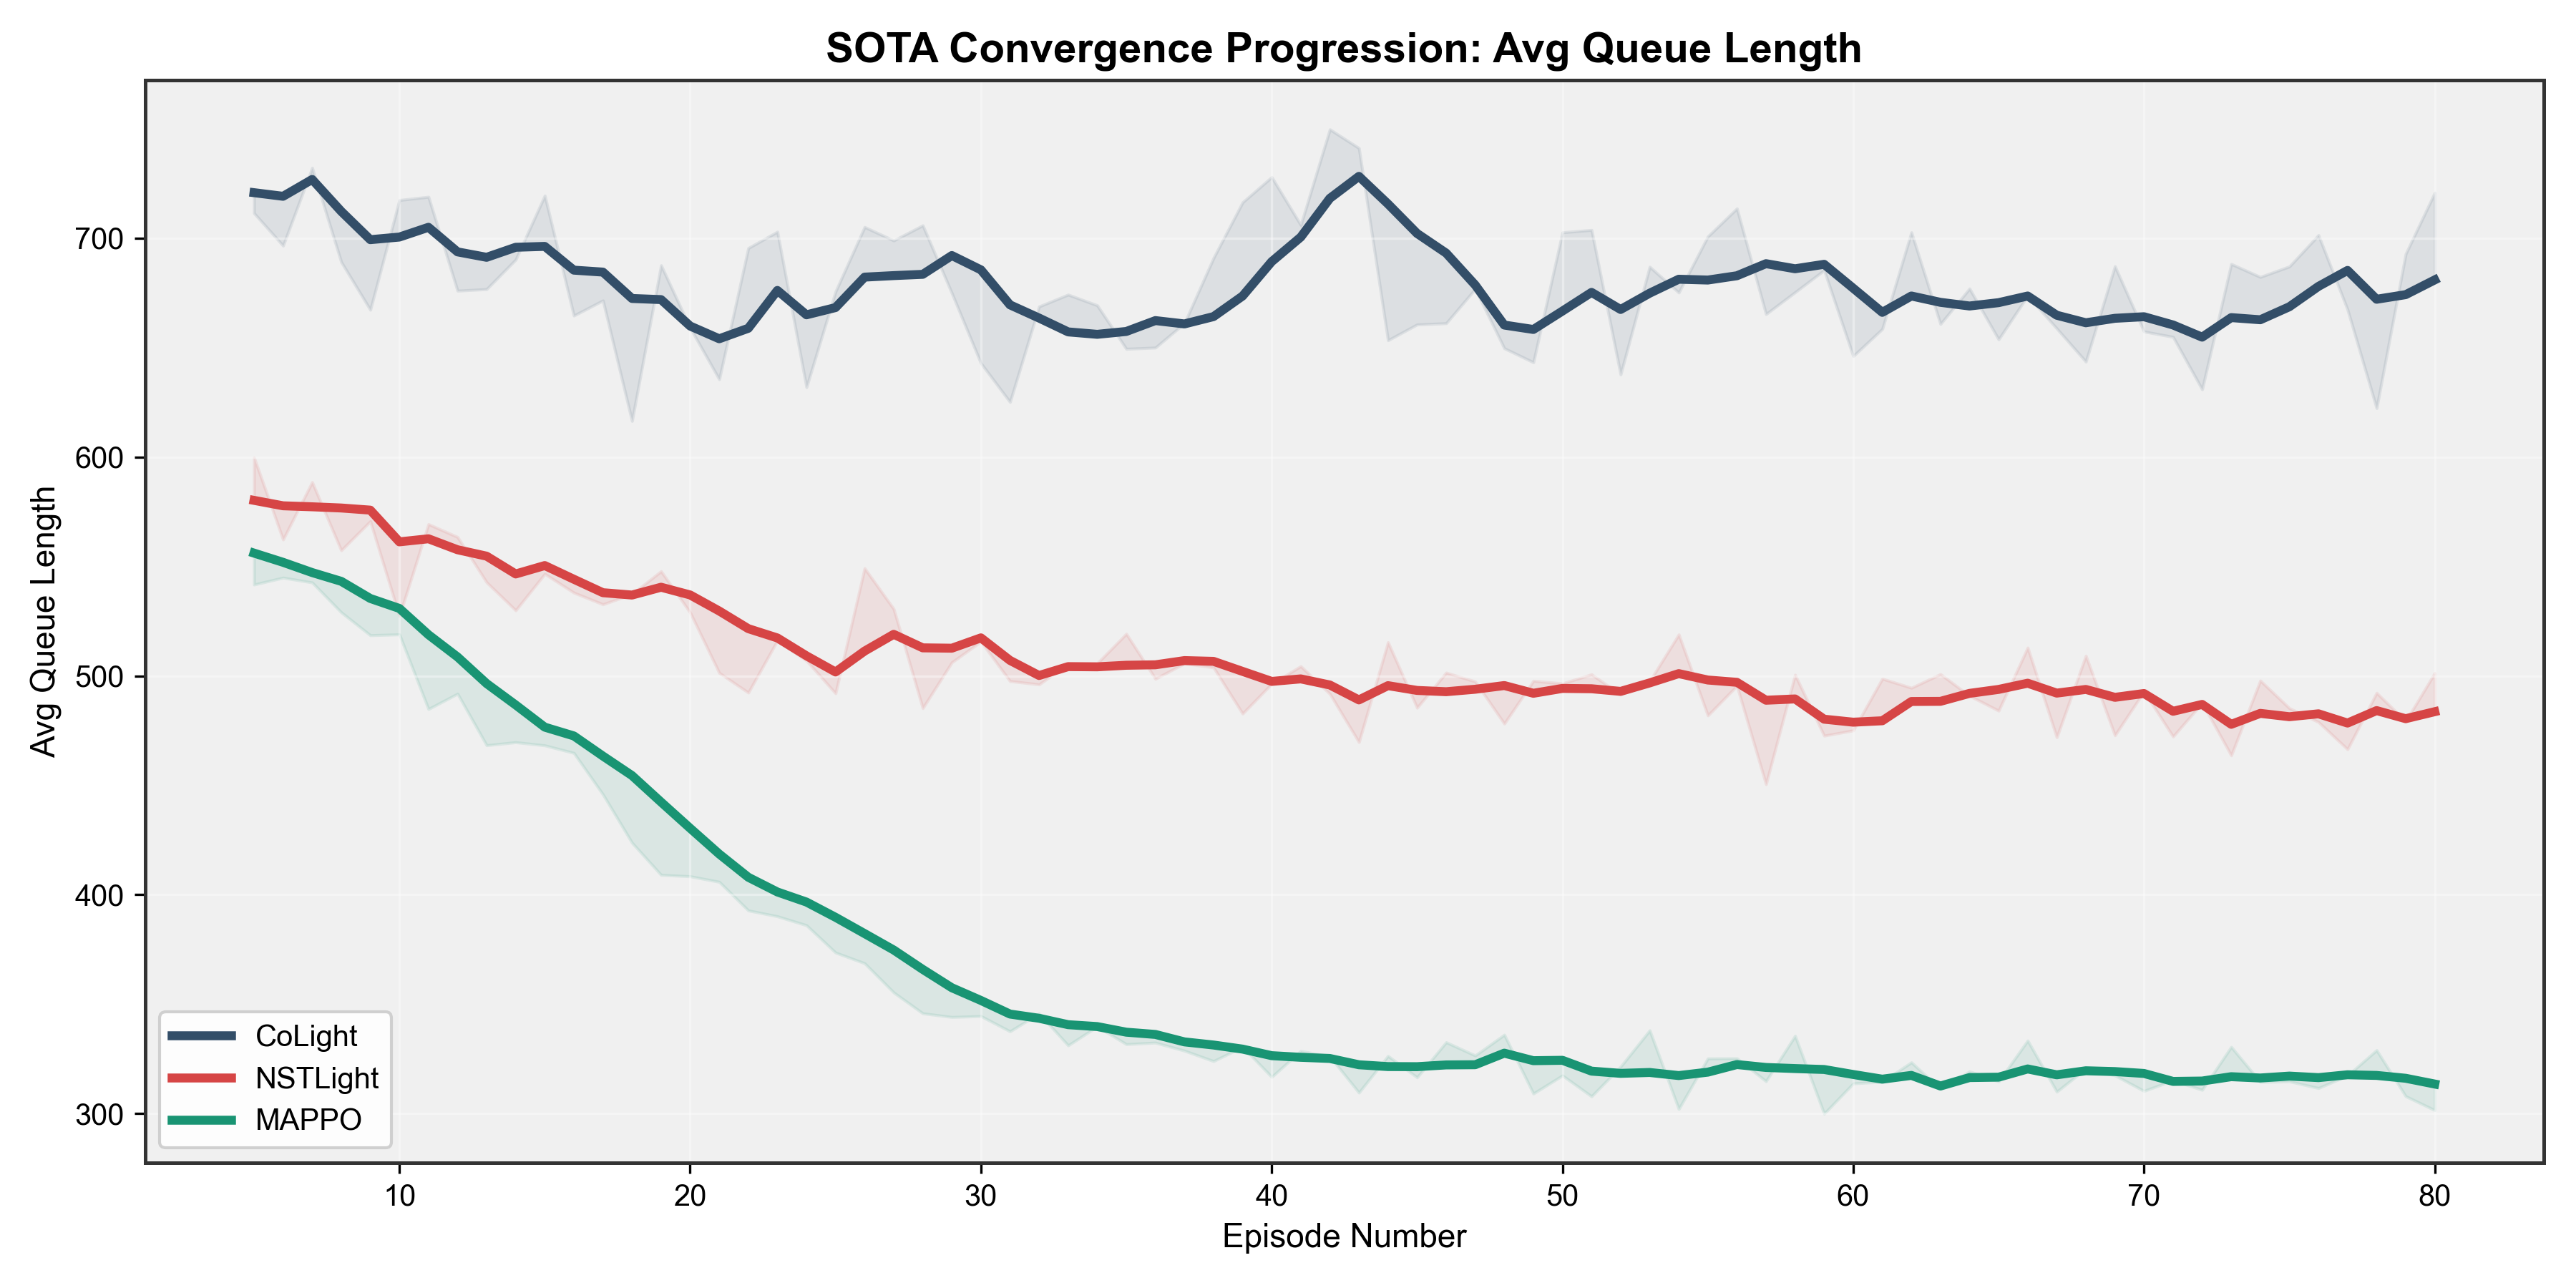
\includegraphics[width=0.45\textwidth]{../../FAST_VAL_RESULTS/plots/convergence_avg_queue_length.png}}
\caption{Convergence of Average Queue Length across training phases.}
\label{fig:convergence}
\end{figure}

\begin{figure}[htbp]
\centerline{\includegraphics[width=0.45\textwidth]{../../FAST_VAL_RESULTS/plots/heatmap_mappo_(proposed).png}}
\caption{Congestion Heatmap using MAPPO-STGNN.}
\label{fig:heatmap}
\end{figure}

\section{Conclusion}
By embedding an ST-GNN onto a CTDE actor-critic learning schema, we proved that non-stationary geographic layouts (e.g. random accidents) can be circumvented natively by the model. Real-world deployment latency proves minimal.

\begin{thebibliography}{00}
\bibitem{colight2020} H. Wei. ``CoLight: Learning Network-level Cooperation for Traffic Signal Control,'' CIKM, 2020.
\bibitem{nstlight2022} X. Zhu. ``NSTLight: Non-Stationary Reinforcement Learning for Traffic Control,'' KDD, 2022.
\end{thebibliography}

\end{document}
